%----------------------------------------------------------------------------------------
%----------------------------------------------------------------------------------------
%----------------------------------------------------------------------------------------
%Method
%----------------------------------------------------------------------------------------
%----------------------------------------------------------------------------------------
%----------------------------------------------------------------------------------------

\section{METHOD}
\label{sec: method}
 \subsection{Self Organizing Maps}
 \label{sec: som}
 
 %Kohonen Self organizing map (or self organizing map, SOM) is an unsupervised neural network for mapping and visualizing a complex and non linear high dimension data introduced by~\citep{Kohonen82}. 
% The SOM is a technique that shows a simple geometry relationship of a non-linear high dimension data on a map \citep{Kohonen98}.
 The SOM is a clustering method which reduces the dimension of data to lower dimensions usually 1 or 2D while preserving topological features of the original data.
 Results of SOM contains nodes (usually hexagonal ones) that arranged in 1D or 2D arrays.
 
 Each nodes may contain one or more samples from input data and distance between nodes represents similarity or dissimilarity of underlying samples. 
 In the way that similar data are closer together in the array and the further nodes go from each other, the more dissimilarity appears between their samples.
 %Sahar_self_notes: maybe "some" is better instead of one or more
 Moreover,a weight vector ``\boldit{W}" with same dimension of the input data associates with each node which will be change during the process and has a key factor in a position of nodes in the map. 
 
 \cite{Geach12} presented the application of the SOM and demonstrate the algorithm of the SOM in detail. In this section we are going to talk briefly about the algorithm of the SOM, how we create our maps and a test model which will help to interpret our results. 
 \subsubsection{Algorithm of SOM} 
 \label{sec: algorithm}
     Assuming we have a data set which contains vectors, \boldit{V} $\in \Re^n$ and we want to map them on S1 by S2 map. 
     We start by creating S1 $\times$ S2 empty neurons. 
     The initial arrangement of these neurons depends on a map's topology provided by user.
     Since the topology of the map does not have any affect on the final result, we chose hexagonal topology which is the default topology for SOMs.
     Then, we assign a random weight vector \boldit{W} $\in \Re^n$ to each node.
     The process of creating SOM, happens over series of $N$ iterations. 
     During each iteration the weight vectors might change according to the Kohonen learning rule (equation~\ref{equ: weight adj}). 
      In each iteration:
     \begin{enumerate}
        \item Choose a random vector from our data set.
        \item Calculate the euclidean distance for each node j as  $D_j^2= \sum_{i=0}^{i=n} (V_i - W_i)^2$, and find a neuron with ``$D_{j_{min}}$". This neuron is the winner node and is calling Best Matching Unit (BMU). 
        \item  Compute the radius of the neighbourhood of the BMU to find nodes within this radius. The weight vectors of these nodes will be affected in the next steps. This value is arbitrary and initially can be set to be as high as half of the SOM size and then it decades exponentially over each iteration:
        \begin{equation}
            r^t_{BMU} = r^0_{BMU}e^{(-t/\tau)}
        \end{equation}
        where $\tau$ is a decay constant and usually set to be the same as number of iterations, $N$. $r^0_{BMU}$ and $r^t_{BMU}$ is the radius of the neighbourhood at 0th and $t$th iteration, respectively. 
        \item Change the weight vectors of the BMU and all the nodes within r(t) as:
        \begin{equation}
            \label{equ: weight adj}
            w(t+1)=w(t)+L(t) \times R(t) \times(v(t)-w(t))
        \end{equation}
        where $L(t) = L_0 e^{(-t/\tau)}$ is the learning factor which prevents divergence of the SOM and $R(t)=exp(-\frac{D_j^2}{2r^t_{BMU}})$ is the influence rate. $R(t)$ determines how weight of nodes in the neighbourhood of BMU will change.
        \item  Repeat these steps for $N$ times.
     \end{enumerate}
     
\subsection{Creating SOM}
\label{sec: create_som}
     In order to create SOM, we used {\tiny MATLAB} neural network toolbox~\citep[NNT,][]{matlabtolbox}.
     SOM in {\tiny NNT} can be created by {\tiny newsom} or {\tiny selforgmap} library which both work in two phases. 
     Phase one is the ``ordering phase". 
     This phase starts with maximum neighbourhood distance, and initial high learning factor usually 0.9 which is provided by user. 
     The ordering phase continues for requested number of iterations and it continues till the learning factor reduces to tuning phase leaning factor and the neighbourhood distance reaches to the number set by the user.
     
     The second phase is the ``tuning phase".
     In this phase the neighbourhood distance is at its minimum, but learning factor decreases very slowly.
     This minimum neighbourhood distance and slowly decreasing the leaning factor helps to fine tune the topology results and causes the more stable SOM. 
     The number of iterations in this tuning phase most be much more than the number iterations in ordering phase, to allow the tuning happens slowly. 
     We chose number of epochs the tuning phase be 3 times more than number of epochs in the ordering phase.
     
     To show our results, we combine two of the {\tiny NNT}'s built-in plots. 
     A Hits map, which shows number of hits for each neurons, and a distances map, which shows the same neurons as the hits map and the distance between them. 
     %To combine these two maps, we wrote number of hits in each neurons in the neurons in a distance map.
     In the maps, the purple hexagonal shape areas represent the neurons.
     %The red lines between neurons, show the immediate neighbours.
     The distances in a distance map are showing by colours.
     The darker colour represents the larger distance between neurons; whilst the lighter colours means there is small distance between neurons.
     In hit maps, neurons with zero hit left empty.
      
    
    %Although size of the SOM could be anything \cite{Vesanto05} suggested that the total number of  $5\sqrt{n}$ neurons provides the most sufficient size.
     Size of SOM maps is arbitrary and there is no rules or restrictions on choosing the size of maps. 
     Users usually must choose the size of grids based on their data set and their usages of the results.
     For training networks using 12 galaxies from K96, we created maps with sizes from $1\times2$ to $50\times50$ to choose the sufficient size.
     varying grids of the maps helps us to monitor whether grouping galaxies in smaller maps is because they have similar SEDs or its because of the shortage of the neurons.
     Based on size of our data and our results, we chose max of the grid size to be 1$\times$22 and 12$\times$12 in 1D and 2D maps, respectively. 
     
     Also for each grid we created different SOM with different, learning factors, neighbourhood distances, and iteration numbers to find the optimize result for our sample.
     Based on our data we created our final SOMs with following initial values: number of iteration in ordering phase = 1000; ordering phase learning factor = 0.9; tuning phase learning factor= 0.02; and tuning phase neighbourhood distance to be 1.
     %All the other parameters are default values in {\tiny newsom} library and cannot be changed by the users. 
     

   
\subsection{Mock sample}
 
         \begin{figure}
            \begin{subfigure}[b]{0.5\textwidth}
                \centering
                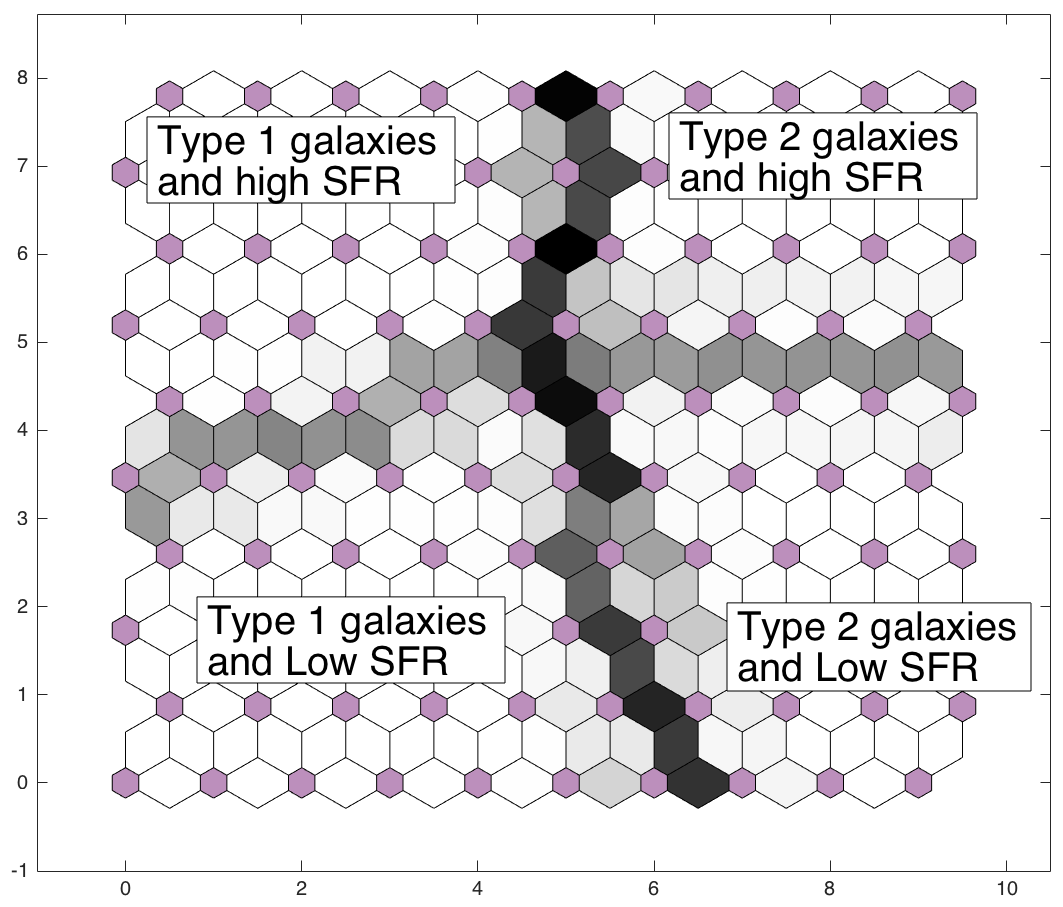
\includegraphics[width=\textwidth]{../images0.01/sample/sample2_dist.png}
            \end{subfigure}
            \hfill
            \begin{subfigure}[b]{0.5\textwidth}
                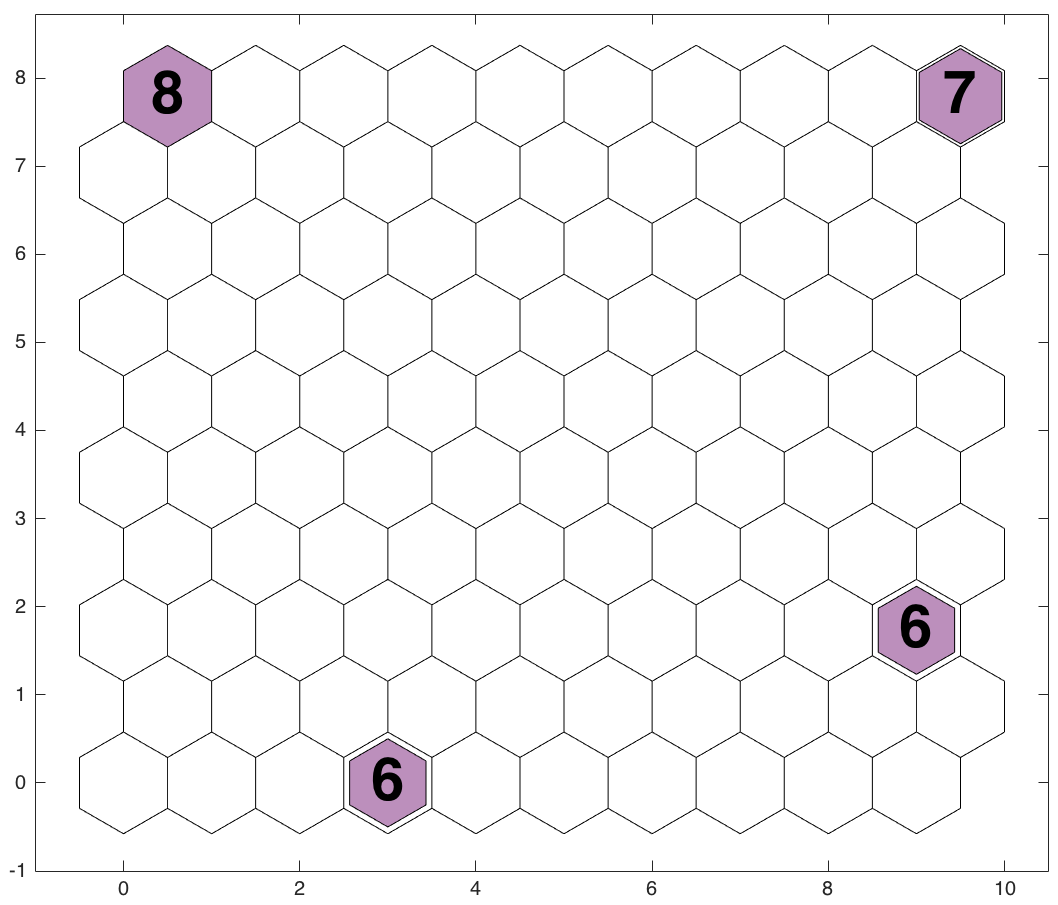
\includegraphics[width=\textwidth]{../images0.01/sample/sample2_hits.png}
            \end{subfigure}
            \caption{SOM of the mock sample. In both plots axis shows the position of the neurones. Hexagonal shapes represent the neurons. The upper plot is a distance map. The gray cycle colours shows the differences between weight of each neuron with white is the minimum differences and black has the maximum one. The lower plot is a hit plot. It represents number of samples in each neurons, while the empty with neurons means zero hit. In this sample the 27 galaxies clustered in 4 groups of 8, 7, 6 and 6 galaxies.}
            \label{fig: sample}
        \end{figure}
 
 We created  a mock sample of 27 galaxies to illustrate the results of SOMs and how they can be analyzed, and to show how this method works.
 The mock sample contains two information from each galaxy; first type of galaxies: type 1 or type 2, and either they are high or low star forming galaxies.
 We generated a SOM with size of $10 \times 10$ using the same initial values mentioned in the Section ~\ref{sec: create_som}.

 Fig. ~\ref{fig: sample} shows the SOM of the mock sample. 
 The upper plot is a distance map. 
 The axis show the position of the neurons in a $10 \times 10$ network. 
 The purple hexagons are illustration of the neurons, and the colours of the area between neighbours are showing the differences between weight of each two neurons.
 In distance maps colour white between neurons represents the minimum value of the differences between weights of neurons and the colour black shows the maximum values. 
 The gray cycle colour between white and black shows values between minimum and maximum with darker colour means more differences.
 
 The lower plot in the Fig.~\ref{fig: sample} shows a hit map.
 In this map similar to the distance map the axis shows the position of the neurons where the hexagonal shapes are neurons.
 %White neurons show the empty neurons.
 The purple neurons with a number on them shows the number of galaxy in that neurons.
 Colour coverage of neurons is different and depends on the number of the hits on the sample.
 The neuron with the maximum number of hits is completely coloured while the empty neurons are white.

Using this method, as we predicted, we were able to divide the mock sample galaxies in 4 distinct groups: Type 1 with high SFR, type 1 with low SFR, type 2 with high SFR and type 2 with low SFR. 
The upper plot in the Fig.~\ref{fig: sample}, clearly shows this division.
The upper part of the plot are high star forming galaxies, while the lower part of it belongs to the low star forming galaxies.
The left part of the plots is where type 1 galaxies belong to and the right side is for type 2 galaxies.
Grey to black colours shows the border between regions.
The lower plot in Fig.~\ref{fig: sample} shows only 4 neurons out of 100 were occupied. 
8 galaxies are type 1 galaxies with high SFR, 7 are type 2 galaxies with high SFR, 6 are type 1 galaxies with low SFR and the other 6 are type 2 galaxies with low SFR. 
The reason of that there are only 4 filled neurons in the network is the simplicity of the input data, and the fact that each entry only could get either 0 or 1 as for type of galaxy and 0 or 0.5 as an indicator of SFR.
It shows us although each galaxy had enough space to occupy any of the neurons in the network, because of the similarity of values they stayed in only four groups. 

As we show in the following sections, in the real world with the real data, we never have two galaxies with exactly the same information.
Therefore, if the network has high enough neurons, the input data would eventually separate from each other and cluster into the smaller and smaller groups. 
However, if the information of the input data are pretty similar to each other, the number of neurons are going to be much higher than number of input samples. 
In similar cases, one can decide that the amount of similarity or dissimilarity between the input samples.



